% Manuel Lippert - Paul Schwanitz
% Physikalisches Praktikum

% Teilaufgabe 1

\section{Allgemeines zum Thema Chaos}
\label{sec:allgemeines}

\subsection{Dynamische Systeme}
\label{sub:dynamSys}
Ein \textit{\textbf{dynamisches System}} ist ein mathematisches Modell eines zeitabhängigen Prozesses, dessen Verlauf nur vom Anfangszustand abhängt. \citep{WikiDynSys}\\
Die Formulierung dieses Sachverhaltes in der Physik geschieht anhand von Differentialgleichungen mit dem Vektor $\vect{x}(t)=(x_1(t)$,..., $x_n(t))\in\mathbb{R}^n$
\begin{gather}
    \dot{\vect{x}}(t)=\vect{F}(\vect{x}(t)),
    \label{eq:dynamDGL}
\end{gather}
dabei beschreibt $\vect{x}(t)$ den \textit{\textbf{Zustand}} des Systems zum Zeitpunkt $t\in\mathbb{R}$.\\
Das dynamische System ist vollständig determiniert, wenn ein Zustand $\vect{x}(t)$ angegeben ist. Aus diesem Zustand lassen sich alle vorangegangen und folgenden Zustände des Systems bestimmen. Dynamische Systeme können auch zeitdiskret angegeben werden, worauf aber hier nicht weiter eingegangen wird. \citep{Lueck}\\

\begin{itemize}
    \item[\textbf{1.}]\textbf{Phasenfluss}\\
    In der Mathematik wird ein dynamisches System durch den \textit{\textbf{Fluss}} bzw. \textit{\textbf{Phasenfluss}}  beschrieben. Unter dem \textit{Fluss} versteht man die Abbildung $\phi:\mathbb{R}^n\times\mathbb{R}\rightarrow\mathbb{R}^n$, welche die \textit{\textbf{Flussaxiome}} erfüllt \citep{Mat1}:
    \begin{gather}
        \begin{aligned}
            (1)~&\phi(\vect{x}_0,0)=\vect{x}_0\\
            (2)~&\phi(\phi(\vect{x}_0,t),s)=\phi(\vect{x}_0,t+s).
            \label{eq:flussaxiome}
        \end{aligned}
    \end{gather}
    Der \textit{Fluss} $\phi$ ordnet \textbf{jedem} Anfangszustand $\vect{x}_0$ einen neuen Zustand zum Zeitpunkt $t$ zu. \citep{Lueck}\\

    \item[\textbf{2.}]\textbf{Trajektorie}\\
    Der \textit{Fluss} $\phi$ kann mit dem \textit{Zustand} $\vect{x}(t)$ in Verbindung gebracht werden mit der Beziehung: $\vect{x}(t)=\phi_{\vect{x}_0}(t)=\phi(\vect{x}_0,t)$ mit festem $\vect{x}$, wobei nach  (\ref{eq:flussaxiome}) $\vect{x}(0)=\phi_{\vect{x}_0}(0)=\phi(\vect{x}_0,0)=\vect{x}_0$ gilt.\\
    Hierbei beschreibt $\phi_{\vect{x}_0}(t)$ die \textit{Lösungskurve}, welche auch \textit{Bahnkurve}, \textit{Orbit}, \textit{Phasenbahn} oder \textit{\textbf{Trajektorie}} des Flusses $\phi$ genannt wird und eine spezielle Lösung von (\ref{eq:dynamDGL}) darstellt, welche wiederum die Bewegung des Punktes $\vect{x}$ unter Wirkung des Flusses $\phi$ mit dem Anfangszustand $\vect{x}_0$ beschreibt. \citep{Lueck}\\
    Durch die Abhängigkeit der \textit{Trajektorien} vom Anfangszustand $\vect{x}_0$ kann gefolgert werden, dass sich \textit{Trajektorien} mit unterschiedlichen Anfangszuständen $\vect{x}_0$ nicht schneiden können. Es können aber unterschiedliche Anfangszustände $\vect{x}_0$ auf derselben \textit{Trajektorie} befinden und sich nur um eine Zeittranslation unterscheiden. \citep{Mat1}\\

    \item[\textbf{3.}]\textbf{Phasenraum}\\
    Der \textit{\textbf{Phasenraum}} oder \textit{\textbf{Zustandsraum}} beschreibt eine Menge aller Zustände oder eine Darstellung aller Trajektorien eines dynamischen Systems und bietet einen Überblick über das Verhalten der gesamten Differentialgleichung ohne diese explizit lösen zu müssen.\\ %!!! Quelle
    %Der \textit{Phasenraum} wird vom Zustand $\vect{x}(t)$ und dessen Ableitung $\dot{\vect{x}}(t)$ aufgespannt bzw. ist eine $(\vect{x}(t),\dot{\vect{x}}(t))$-Ebene, was eine Parameterdarstellung der Differentialgleichung über die Zeit $t$ darstellt.
    %In diesem \textit{Phasenraum} lässt sich dann ein Vektor $(\vect{x},\dot{\vect{x}})$ definieren, welcher auf die \textit{Trajektorien}, die sich mit dem Anfangszustand $\vect{x}_0$ änderen, zeigt. Die Ableitung dieses Vektors $\frac{\text{d}}{\text{d}t}(\vect{x},\dot{\vect{x}})=(\dot{\vect{x}},\ddot{\vect{x}})$ erzeugt ein \textit{Vektorfeld} bzw. ein \textit{Richtungsfeld} der Differentialgleichung, dessen Vektoren tangential auf den \textit{Trajektorien} steht.

    \item[\textbf{4.}]\textbf{Attraktor}\\
    In (\ref{eq:dynamDGL}) wird ein Vektorfeld $\vect{F}$ im Phasenraum definiert, welches als Geschwindigkeitfeld des Phasenflusses $\phi$ angesehen werden kann.\\ Durch Betrachtung der Divergenz des Vektorfelds $\nabla\vect{F}$ kann eine Aussage getroffen werden über die Rate mit dem sich ein Volumenelement $V$ unter der Wirkung des Flusses verändert. Zwei Fälle sind hier besonders hervorzuheben:
    \begin{gather}
        \begin{aligned}
            (1)~&\nabla\cdot\vect{F}=0\Rightarrow \dot{V}=0 \Rightarrow~\text{Konservatives System}\\
            (2)~&\nabla\cdot\vect{F}<0\Rightarrow \dot{V}<0 \Rightarrow~\text{Dissipatives System}
        \end{aligned}
    \end{gather}
    In einem dissipativen System laufen die Trajektorien nach einer Einlaufsphase (transiente Bewegung) in einem begrenzten Bereich im Phasenraum, welchen man als \textit{\textbf{Attraktor}} bezeichnet (Bewegung auf \textit{Attraktor}: permante oder posttransiente Bewegung). Ein Attraktor weist folgende Eigenschaften auf:
    \begin{itemize}
        \item[(1)] Kompakte Menge im Phasenraum
        \item[(2)] Invariant unter der Wirkung des Flusses
        \item[(3)] Volumen des Attraktors ist Null
        \item[(4)] Eine beliebige Obermenge des Attraktors schrumpft unter der Wirkung des Flusses auf den Attraktor selbst zusammen   
    \end{itemize}
    \textbf{Arten von Attraktor}
    \begin{center}
        \begin{tabular}{ccc}
            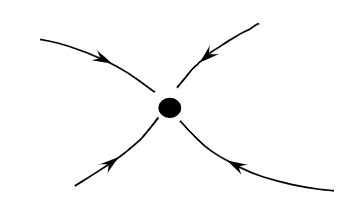
\includegraphics[width=4cm]{FixpunktAttraktor.png}
            & 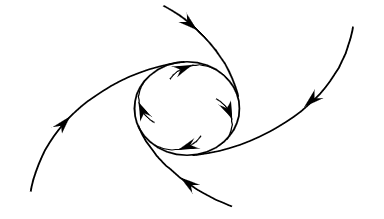
\includegraphics[width=4cm]{GrenzzyklusAttraktor.png}
            & 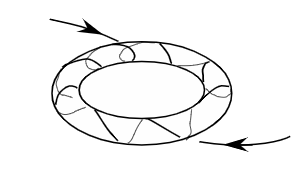
\includegraphics[width=4cm]{TorusAttraktor.png}
        \end{tabular}
        \captionof{figure}{Fixpunkt, Grenzzyklus, Tours- bzw. Ringattraktor}
        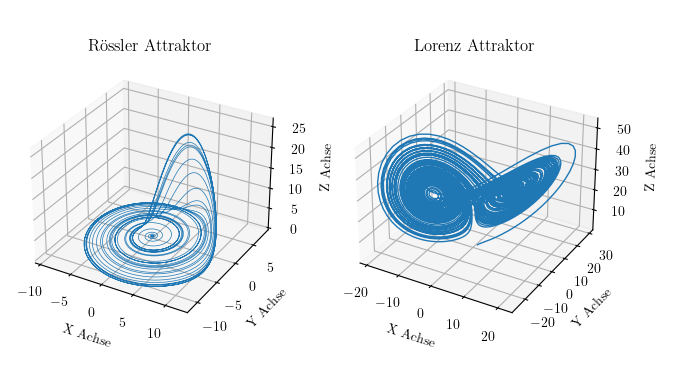
\includegraphics[width=14cm]{SeltsameAttraktoren.png}
        \captionof{figure}{Seltsame Attraktoren: Rössler- und Lorentzattraktor}
    \end{center}
    % !!! Quelle \citep{Lueck}
\end{itemize}

\subsection{Deterministisches Chaos}
\label{sub:determChaos}
% TODO: #17 FzV 2.1.3 @PaulSchwanitz

\subsection{Fouriertransformation und Leistungsspektrum}
\label{sub:fouriertrafo}
% TODO: #19 FzV 2.1.4 @PaulSchwanitz

\subsection{Darstellungsweisen eines chaotischen Attraktor}
\label{sub:darstellungAttraktor}
\begin{itemize}
    \item[\textbf{1.}]{\textbf{Phasenraumdarstellung}}\\
    Die \textit{\textbf{Phasenraumdarstellung}} wie in \ref{sec:allgemeines} erwähnt, gibt einen Überblick über den Verlauf der Bewegung des dynamischen Systems. Dabei trägt man je an eine Raumachse eine Phasenraumvariabel auf (z.B. $x, \dot{x}$), wobei der Phasenraum dabei $n$-Dimensionen haben kann und nicht alle Phasenraumvariablen bekannt sein müssen, da ein Attraktor im Phasenraum rekonstruiert werden kann. Dazu werden die Messwerte einer Phasenraumvariablen bei einer festen Zeitspanne $\tau$, also $\varphi(t), \varphi(t+\tau)$,..., $\varphi(t+(n-1)\tau)$, als neu Koordinaten $x_i$ (z.B. $x_1=\varphi(t) und x-2=\varphi(t+\tau))$ eines neuen Koordinatensystems. Bei richtiger Wahl von $\tau$ und $n$ lässt sich der tatsächliche Attraktor rekonstruieren. \citep{Lueck}
    \item[\textbf{2.}]{\textbf{Poincar\'e-Abbildung}}\\
    Die \textit{\textbf{Poincar\'e-Abbildung}} ist eine Projektion des \textit{\textbf{Poincar\'e-Schnitts}} an einer Ebene. Diese Abbildung ist immer die Dimension $n-1$ und ist somit eine Dimension niedriger als der Phasenraum mit der Dimension $n$ und es gehen keinen Informationen bzgl. dem Langzeitverhalten des Systems verloren. Aufgrund dieser Tatsache lässt sich die \textit{Poincar\'e-Abbildung} zur Analyse von höherdimensionalen Phasenräumen verwenden. Der \textit{Poincar\'e-Schnitt} ist dabei eine Menge aller Durchstoßpunkte der Trajektorien im Phasenraum auf einer Hyperfläche. Hierbei müssen die Trajektorien die Hyperfläche \textit{transversal} (senkrecht) und in einer vorgegebenen Richtung schneiden. Praktisch werden meistens die Lage von Extremwerten einer Messgröße als Bedingung für die Schnittebene (Hyperfläche) und trägt diese gegen die anderen Phasenraumvariablen zu diesem Zeitpunkt gegeneinander auf oder man wählt eine Ebene, die den Attraktor geeignet schneidet. \citep{Lueck}
    \item[\textbf{3.}]{\textbf{Wiederkehr-Abbildung}}\\
    Bei der \textit{\textbf{Wiederkehr-Abbildung}} wird eine diskrete Abbildung aktueller Messwerte über die vorangegangenen Messwerte augetragen. Diese Abbildung ähnelt dann einen \textit{Poincar\'e-Schnitt}, weswegen man bei einem kontinuierlichen System (\ref{eq:dynamDGL}) dessen \textit{Poincar\'e-Abbildung} für dieses Verfahren verwendet. \citep{Lueck}
    \item[\textbf{4.}]{\textbf{Bifurkationsdiagramm}}\\
    Bei einem \textit{\textbf{Bifurkationsdiagramm}} betrachtet man die Projektion der \textit{Poincar\'e-Abbildung} auf \textbf{eine} Achse unter Veränderung eines Kontrollparameters (z.B. der Zeit $t$), wobei man die durch die Projektion gewonnenen Werte gegen den jeweiligen Parameterwert aufträgt. \citep{Lueck}
    \item[\textbf{5.}]{\textbf{Phasendiagramm}}\\
    Wenn bei dem \textit{Bifurkationsdiagramm} mehrere unterschiedliche voneinander unabhängige Parameter existieren, verwendet man das \textit{\textbf{Phasendiagramm}}. Dazu trägt man die als Koordinaatenachsen die jeweiligen Parameter, die das Systemverhalten beeinflussen, gegeneinander auf und erhält Landkarte des globalen Systemverhaltens in Abhängigkeit der gewählten Parameter. \citep{Lueck}    
\end{itemize}